\documentclass[../main/main.tex]{subfiles}

\newdate{date}{27}{03}{2020}

\begin{document}

\marginpar{ \textbf{Lecture 6.} \\  \displaydate{date}. \\ Compiled:  \today.\vspace{0.5cm}}

\subsubsection{First order correction \(\pmb{\hat{H}_1}\)}

Now, let us evaluate the first order correction term. Clearly, in the perturbative approach, the \textbf{first order correction} term \marginpar{First order correction} is obtained just by taking the matrix element of the potential energy term between the non-interacting Fermi ground state:
\begin{equation*}
  E^{(1)} = \bra{F} \hat{H}_1 \ket{F}
  = \frac{e^2}{2V} \sum_{\va{k}\va{p}\va{q}}^{'} \sum_{\lambda \mu }^{} \frac{4 \pi }{q^2} \bra{F} a_{\va{k} + \va{q}, \lambda }^\dag a_{\va{p}- \va{q}, \mu } ^\dag a_{\va{p} \mu } a_{\va{k} \lambda } \ket{F}
\end{equation*}
where we have
\begin{equation*}
  a_{\va{p} \mu } a_{\va{k} \lambda } \ket{F}  \neq 0 \quad  \text{ only if } \abs{\va{k}} \le k_F, \abs{\va{p}} \le k_F
\end{equation*}
and
\begin{equation*}
  \bra{F} a_{\va{k} + \va{q}, \lambda }^\dag a_{\va{p}- \va{q}, \mu } ^\dag = \qty(  a_{\va{p}- \va{q}, \mu } a_{\va{k} + \va{q}, \lambda } \ket{F} ) ^\dag \neq 0
  \quad  \text{ only if } \abs{\va{k} + \va{q}} \le k_F, \abs{\va{p} - \va{q}} \le k_F
\end{equation*}
where the condition is such that the wave vectors are inside the Fermi sphere.
Hence the matrix element \( \bra{F} \hat{H}_1 \ket{F}    \) can be different from zero only if certain conditions apply. In particular, the first two destruction operators \(   a_{\va{p} \mu } a_{\va{k} \lambda } \) destroy two particles while the other two creation operators \( a_{\va{k} + \va{q}, \lambda }^\dag a_{\va{p}- \va{q}, \mu } ^\dag  \) create two particles and, in order that the action of these last two creation operators gives a result different from zero, they should act on an empty state.
More specifically, the matrix element can be different from zero only if the two creation operators exactly fill up the holes made by the two destruction operators, namely two particles are destroyed and then two additional particles are created in exactly the same state inside the Fermi sphere.
By considering the wave vector index of these operators, there are only two possibilities:
\begin{equation*}
  \begin{cases}
   \va{k}+\va{q} = \va{k} &(\lambda = \lambda )\\
   \va{p}-\va{q} = \va{p} &(\mu = \mu )
  \end{cases}
  \quad \quad \quad
  \begin{cases}
   \va{k}+\va{q} = \va{p} & (\lambda = \mu )\\
   \va{p}-\va{q} = \va{k} & (\mu = \lambda )
  \end{cases}
\end{equation*}
where the the contribution on the left is called \textbf{direct term} while the one on the right \textbf{exchange term}. \marginpar{Direct and exchange term \vspace{0.5cm}}
The direct term realizes only if  \( \va{q}=0 \), but  in the sum \( \sum_{}^{'}   \) the \( \va{q}=0 \) term is not considered. Hence, in our specific case, the condition in the direct term is not possible. \marginpar{
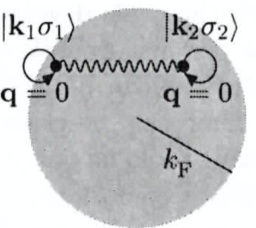
\includegraphics[width=0.95\marginparwidth]{../lessons/6_image/3.png}
\captionof{figure}{\label{fig:} Direct interaction.}
}
\marginpar{
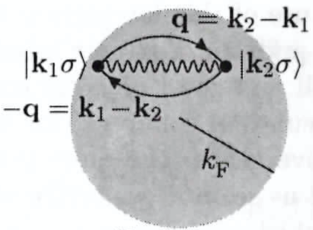
\includegraphics[width=\marginparwidth]{../lessons/6_image/4.png}
\captionof{figure}{\label{fig:} Exchange interaction.}
}
On the contrary, the condition of the exchange term can be realized. It is called exchange term, because if we interpreted \( \va{q} \) as a wave vector, or momentum, there is momentum transferred from one particle to another one. Moreover, this case is applicable if we consider interactions only between electrons with equal spins, \( \delta _{\lambda , \mu } \).
In practice, this means that the only possibility is:
\begin{equation*}
\begin{split}
  E^{(1)} &= \frac{e^2}{2V} \sum_{\va{k}\va{q}, \lambda }^{'}
  \frac{4 \pi }{q^2}
  \bra{F} a_{\va{k} + \va{q}, \lambda }^\dag \mathcolorbox{green!20}{a_{\va{k}, \lambda  } ^\dag a_{\va{k}+\va{q}, \lambda  }} a_{\va{k} \lambda } \ket{F}
   \\
   & =
   \frac{e^2}{2V} \sum_{\va{k}\va{q}, \lambda }^{'}
   \frac{4 \pi }{q^2}
   \bra{F} a_{\va{k} + \va{q}, \lambda }^\dag   \mathcolorbox{green!20}{\qty(- a_{\va{k}+\va{q}, \lambda } a_{\va{k}\lambda }^\dag  + \underbrace{\delta _{\va{k},\va{k}+\va{q}}}_{=0 \, (\va{q}\neq0)} )} a_{\va{k} \lambda } \ket{F}
\end{split}
\end{equation*}
where the green transforms due to the anticommutation rule and where the \( \delta  \) is different from zero only if \( \va{q}=0 \).  Hence, since in our case the \( \va{q}=0  \) term is not present, the \( \delta  \) gives no contribution (in practice, we can interchange these two operators by adding a minus sign).
By replacing the destruction and creation operator with the number ones:
\begin{equation*}
  E^{(1)} = -\frac{e^2}{2V} \sum_{\substack{\va{k}\va{q}, \lambda  \\ \abs{\va{k}} \le k_F, \abs{\va{k}+\va{q}}\le k_F   } }^{'}
\frac{4 \pi }{q^2} \bra{F} \hat{n}_{\va{k}+\va{q},\lambda } \hat{n}_{\va{k}\lambda } \ket{F}  <0!
\end{equation*}
this exchange term results negative even though the electron-electron interaction is repulsing. It is called \textbf{Hartree-Fock} approximation, for a homogeneous system. \marginpar{Hartree-Fock approximation}
Now, we should try to really evaluate this expression. First of all, we observe that:
\begin{equation*}
  \begin{cases}
  \hat{n}_{\va{k} \lambda } =\ket{F} & \text{if } \abs{\va{k}}\le k_F   \\
  \hat{n}_{\va{k}+\va{q}, \lambda } =\ket{F} & \text{if } \abs{\va{k}+\va{q}}\le k_F
  \end{cases}
\end{equation*}
because by construction \( \va{k} \) and \( \va{k} + \va{q} \) are in the Fermi sphere.
Therefore, we get:
\begin{equation*}
  E^{(1)} = -\frac{e^2}{2V} \sum_{\substack{\va{k}\va{q}, \lambda  \\ \abs{\va{k}} \le k_F, \abs{\va{k}+\va{q}}\le k_F   } }^{'} \frac{4 \pi }{q^2}
  \underset{L \rightarrow \infty }{\longrightarrow }
  - \frac{\mathcolorbox{yellow!40}{2}e^2}{2V} \frac{V^2}{(2 \pi )^6}
  \int_{}^{} \dd[]{\va{k}}
  \int_{}^{} \dd[]{\va{q}} \frac{4 \pi }{q^2} \Theta (k_F- k) \Theta (k_F - \abs{\va{k}+\va{q}} )
\end{equation*}
where by considering the thermodynamic limit we compute integrals instead of sums (it is simpler), going from a double sum to a double integral. In particular, we get the yellow term "2" by summing over \( \lambda  \) and  the \( \theta  \) functions are introduced to enforce the conditions in the sums. Moreover, \( \va{q} \neq 0 \) can be omitted since it effects the integrand at only a single point, so it is negligible compared to the rest of the contribution.

Now it is convenient to make the expression more symmetric. For that purpose, we introduce new variables:
\begin{equation*}
  \va{p} \equiv \va{k} + \frac{\va{q}}{2} \quad \Rightarrow \va{k} = \va{p}-\frac{\va{q}}{2}
\end{equation*}
Thus we obtain:
\begin{equation*}
  E^{(1)} = - \frac{4 \pi e^2 V}{(2 \pi )^6}
  \int_{}^{} \dd[]{\va{q}} \frac{1}{q^2}
  \int_{}^{} \dd[]{\va{p}} \Theta \qty(k_F - \abs{\va{p}-\frac{\va{q}}{2}} )
  \Theta \qty(k_F - \abs{\va{p}+ \frac{\va{q}}{2}} )
\end{equation*}
and considering that \( \abs{\va{p}\pm \frac{\va{q}}{2}} \le k_F \), the region of integration over \( \va{p} \) is the intersection between 2 spheres of radius \( k_F \). Indeed, it is easy to demonstrate that you can have a non vanishing contribution only if \( \abs{\va{q}}\le 2 k_F  \).
Hence, this integral is equal to compute the volume of the intersection between two spheres of radius \( k_F \) (see Fig.\ref{fig:6_2}) that are located in a such a way that the distance between their centers is exactly given by \( \va{q} \). Thus we have reduced an integral to a geometrical problem by evaluating the intersection between two spheres at distance \( \va{q} \).

\begin{figure}[h!]
\centering
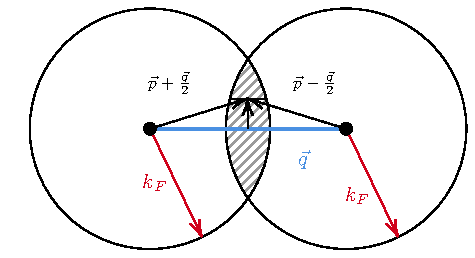
\includegraphics[width=0.7\textwidth]{../lessons/6_image/2.pdf}
\caption{\label{fig:6_2} Intersection between two spheres of radius \( k_F \) at distance \( \abs{\va{q}}  \le 2 k_F\).}
\end{figure}


It is convenient to go to dimensionless variables:
\begin{equation*}
  x \equiv \frac{q}{2k_F}
\end{equation*}
Hence:
\begin{equation*}
\begin{split}
  \int_{}^{}   \frac{\dd[]{\va{q}}}{q^2} \int_{}^{} \dd[]{\va{p}}  \Theta \qty(k_F - \abs{\va{p}-\frac{\va{q}}{2}} ) &\Theta \qty(k_F - \abs{\va{p}+ \frac{\va{q}}{2}} )  =
    \int_{}^{} \frac{\dd[]{\va{q}}}{q^2}
  \frac{4 \pi k_F^3}{3}  \qty(1 - \frac{3}{2}x + \frac{x^3}{2}) \Theta (1-x)  \\
  &= 4 \pi\int_{0}^{\infty } \dd[]{q} \frac{\cancel{q^2}}{\cancel{q^2}} \qty[
  \frac{4 \pi k_F^3}{3}  \qty(1 - \frac{3}{2}x + \frac{x^3}{2}) \Theta (1-x)] \\
  &= 4 \pi 2 k_F \int_{0}^{\infty } \dd[]{q} \frac{1}{2k_F} \qty[
  \frac{4 \pi k_F^3}{3}  \qty(1 - \frac{3}{2}x + \frac{x^3}{2}) \Theta (1-x)] \\
  & = 4 \pi  2 k_F \int_{0}^{\infty } \dd[]{x} \qty[
  \frac{4 \pi k_F^3}{3}  \qty(1 - \frac{3}{2}x + \frac{x^3}{2}) ] \Theta (1-x) \\
  & = 4 \pi  2 k_F \int_{0}^{1} \dd[]{x}  \qty[
  \frac{4 \pi k_F^3}{3}  \qty(1 - \frac{3}{2}x + \frac{x^3}{2}) ]
\end{split}
\end{equation*}
The first correction term results:
\begin{equation*}
\begin{split}
E^{(1)} &= - \frac{4 \pi e^2 V}{(2 \pi )^6} (4 \pi  2 k_F) \frac{4 \pi k_F^3}{3} \underbrace{\qty[ \int_{0}^{1} \dd[]{x}   \qty(1 - \frac{3}{2}x + \frac{x^3}{2})  ]}_{= 3/8}   \\
& = \frac{2}{3} \frac{e^2V}{\pi ^3}k_F^3 k_F \qty(\frac{3}{8})
\overset{(a)}{=} \frac{2 e^2 N}{\pi } \qty(\frac{9 \pi }{4})^{1/3} \frac{1}{r_s a_0} \qty(\frac{3}{8}) \\
&= - \qty(\frac{e^2}{2 a_0}) \frac{N}{r_s} \underbrace{\qty[\qty(\frac{9 \pi }{4})^{1/3} \frac{3}{2 \pi } ]  }_{=0.916}
\end{split}
\end{equation*}
where in the step \( (a) \) we have made the substitutions:
\begin{equation*}
  k_F^3 = 3 \pi ^2 \frac{N}{V} \quad \quad k_F = \qty(\frac{9 \pi }{4})^{1/3} \frac{1}{r_s a_0}
\end{equation*}
By substituting the numerical result we have:
\begin{equation}
  E^{(1)} = - \underbrace{\qty(\frac{e^2}{2 a_0})}_{=1 \text{Ryd}}  \frac{N}{r_s} \vdot 0.916 < 0
\end{equation}
so the first order correction (exchange or Hartree-Fock term) is negative as anticipated.

Now, the question is how  we can interpret this contro-intuitive fact from a physical point of view, namely the reason why the electron-electron interaction gives a negative contribution to the energy.
Since mathematically the the minus sign rise due to the antisymmetry of the wave functions, the physical origin is the Pauli exclusion principle, which prevents two electrons with parallel spin from getting too close.
More specifically, we can visualize the situation as follow (see Fig.\ref{fig:6_1}): \marginpar{
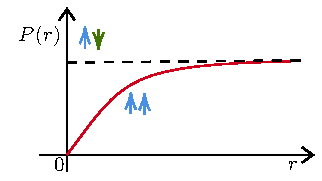
\includegraphics[width=\marginparwidth]{../lessons/6_image/1.pdf}
\captionof{figure}{\label{fig:6_1} Probability of finding an electron at the distance \( r \), for parallel and antiparallel spins.}
} suppose that we put an electron in the origin and we want to look at the probability of finding another electron at a certain distance \( r \). If we consider an independent particle approach and suppose that electrons have parallel spins, since there is no interaction term the probability of finding the electron at the distance \( r \) is uniform (i.e. the same at all the distances). However, we are considering electrons with parallel spins hence, even if there is no direct Coulomb interaction acting on the system, in any case there is the Pauli exlusion principle: we cannot have the two electrons with parallel spins occupy the same position or even very close to each other. This produced the so called \textbf{exchange-hole} concept,\marginpar{Exchange-hole} which means that the probability of finding another electron with same spin very close to the given electron is reduced with respect to the situation where the Pauli principle where not active.

In other words, the electrons are forced somehow to avoid each other since only one electron at a time can be at a given point in space: the "direct" classical Coulomb interaction (\( \va{q}=0 \)) does not take this into account (it was just used to cancel divergences) and overstimates the energy while the "exchange" part correct for this by being negative.
In other words, while a direct classical term does not take Pauli exclusion principle into account and tend to overstimate the energy, the exchange part corrects for this and gives a negative contribution.
This is the reason why we really get a minus sign for this contribution to the energy.

In Fig.\ref{fig:6_3} are shown some pictures to have a better idea of what is happening. In particular, on the right there is the Fermi sphere, on the left it is projected just along one dimension and the states are occupied up to the Fermi level.

\begin{figure}[h!]
\begin{minipage}[c]{0.5\linewidth}
\centering
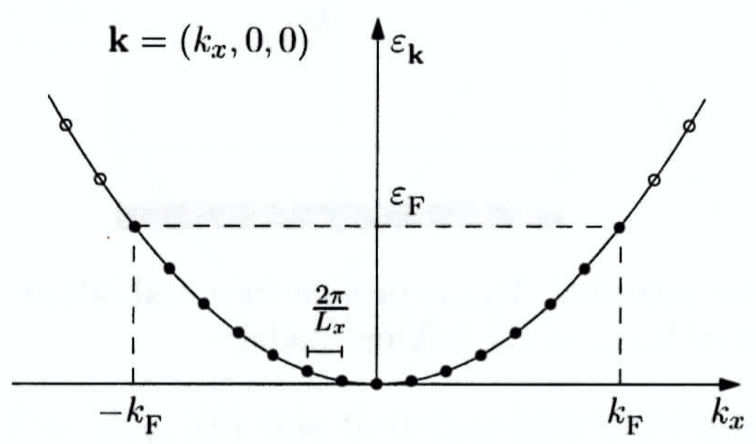
\includegraphics[width=0.9\textwidth]{../lessons/6_image/5.png}
\end{minipage}
\begin{minipage}[]{0.5\linewidth}
\centering
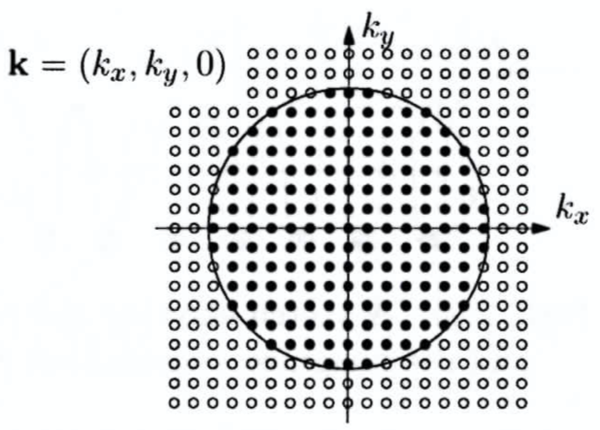
\includegraphics[width=0.8\textwidth]{../lessons/6_image/6.png}
\end{minipage}
\caption{\label{fig:6_3} Two aspects of \( \ket{F}  \) in \( \va{k} \)-space. To the left the disperion relation \( \varepsilon _{\va{k}} \) is plotted along the line \( \va{k}=(k_x,0,0) \) and \( \varepsilon _F \) and \( k_F \) are indicated. To the right the occupation of the states is shown in the plane \( \va{k}=(k_x,k_y,0) \). The Fermi sphere is shown as a circle with radius \( k_F \). Filled and empy circles represent occupied and unoccupied states, respectively.}
\end{figure}


\subsubsection{Jellium model: final results and comments}

To summarize, we have seen that in the high density limit (\( r_s \rightarrow 0 \)), the total energy of the Jellium system is given by:
\begin{equation*}
  E = E_0 + E^{(1)} + \dots
\end{equation*}
Thus, the energy per particle is:
\begin{equation*}
  \frac{E}{N}  \underset{r_s \rightarrow 0}{=} \qty(\frac{e^2}{2 a_0}) \qty[ \mathcolorbox{yellow!40}{\frac{2.21}{r_s^2}}- \mathcolorbox{green!20}{\frac{0.916}{r_s}}+\dots]
\end{equation*}
where the yellow term correspond to the kinetic energy term, while the green one the Hartree-Fock exchange energy term. Of course, in principle, we have an infinite series of terms; all the remaining terms are denoted by the definition of Wigner (1933) as \marginpar{Correlation energy}  \textbf{correlation energy}. This historical definition is misleading, because in principle also the Hartree-Fock exchange energy has to do with some sort of correlations between the electrons. Another definition is given by Feymann (1972) that called all the remaining terms \textbf{stupidity energy}, because of the difficulty to go beyond the Hartree-Fock term in order of expansion.

Let us consider only the first two terms; hence, the energy per particle at the first order in the high density limit results:
\begin{equation*}
  \frac{E}{N} \underset{r_s \rightarrow 0}{\simeq }
  \qty(\frac{e^2}{2 a_0}) \qty[ \frac{2.21}{r_s^2}- \frac{0.916}{r_s}]
\end{equation*}
It is interesting to consider \( E/N \) as a function of \( r_s \) as in Fig.\ref{fig:6_4}. We can note that the dominant term as \( r_s \rightarrow 0\) is the kinetic energy term, while the exchange term is the dominant  one if \( r_s \) is large. The combination of the two contribution is the solid line in orange. In particular, this curve has a \emph{minimum} for a negative value of the energy and for a given value of \( r_s \). Physically, it means that the system is stable system and bounded which explains why the metals are stable. One should remember that while in the vanishing \( r_s \rightarrow 0 \) region the exact solution is the one founded, we cannot say the same for relatively large value of the \( r_s \) parameter. Indeed, even around the minimum the result is just an approximation because we stopped at the first order term.

\begin{figure}[h!]
\centering
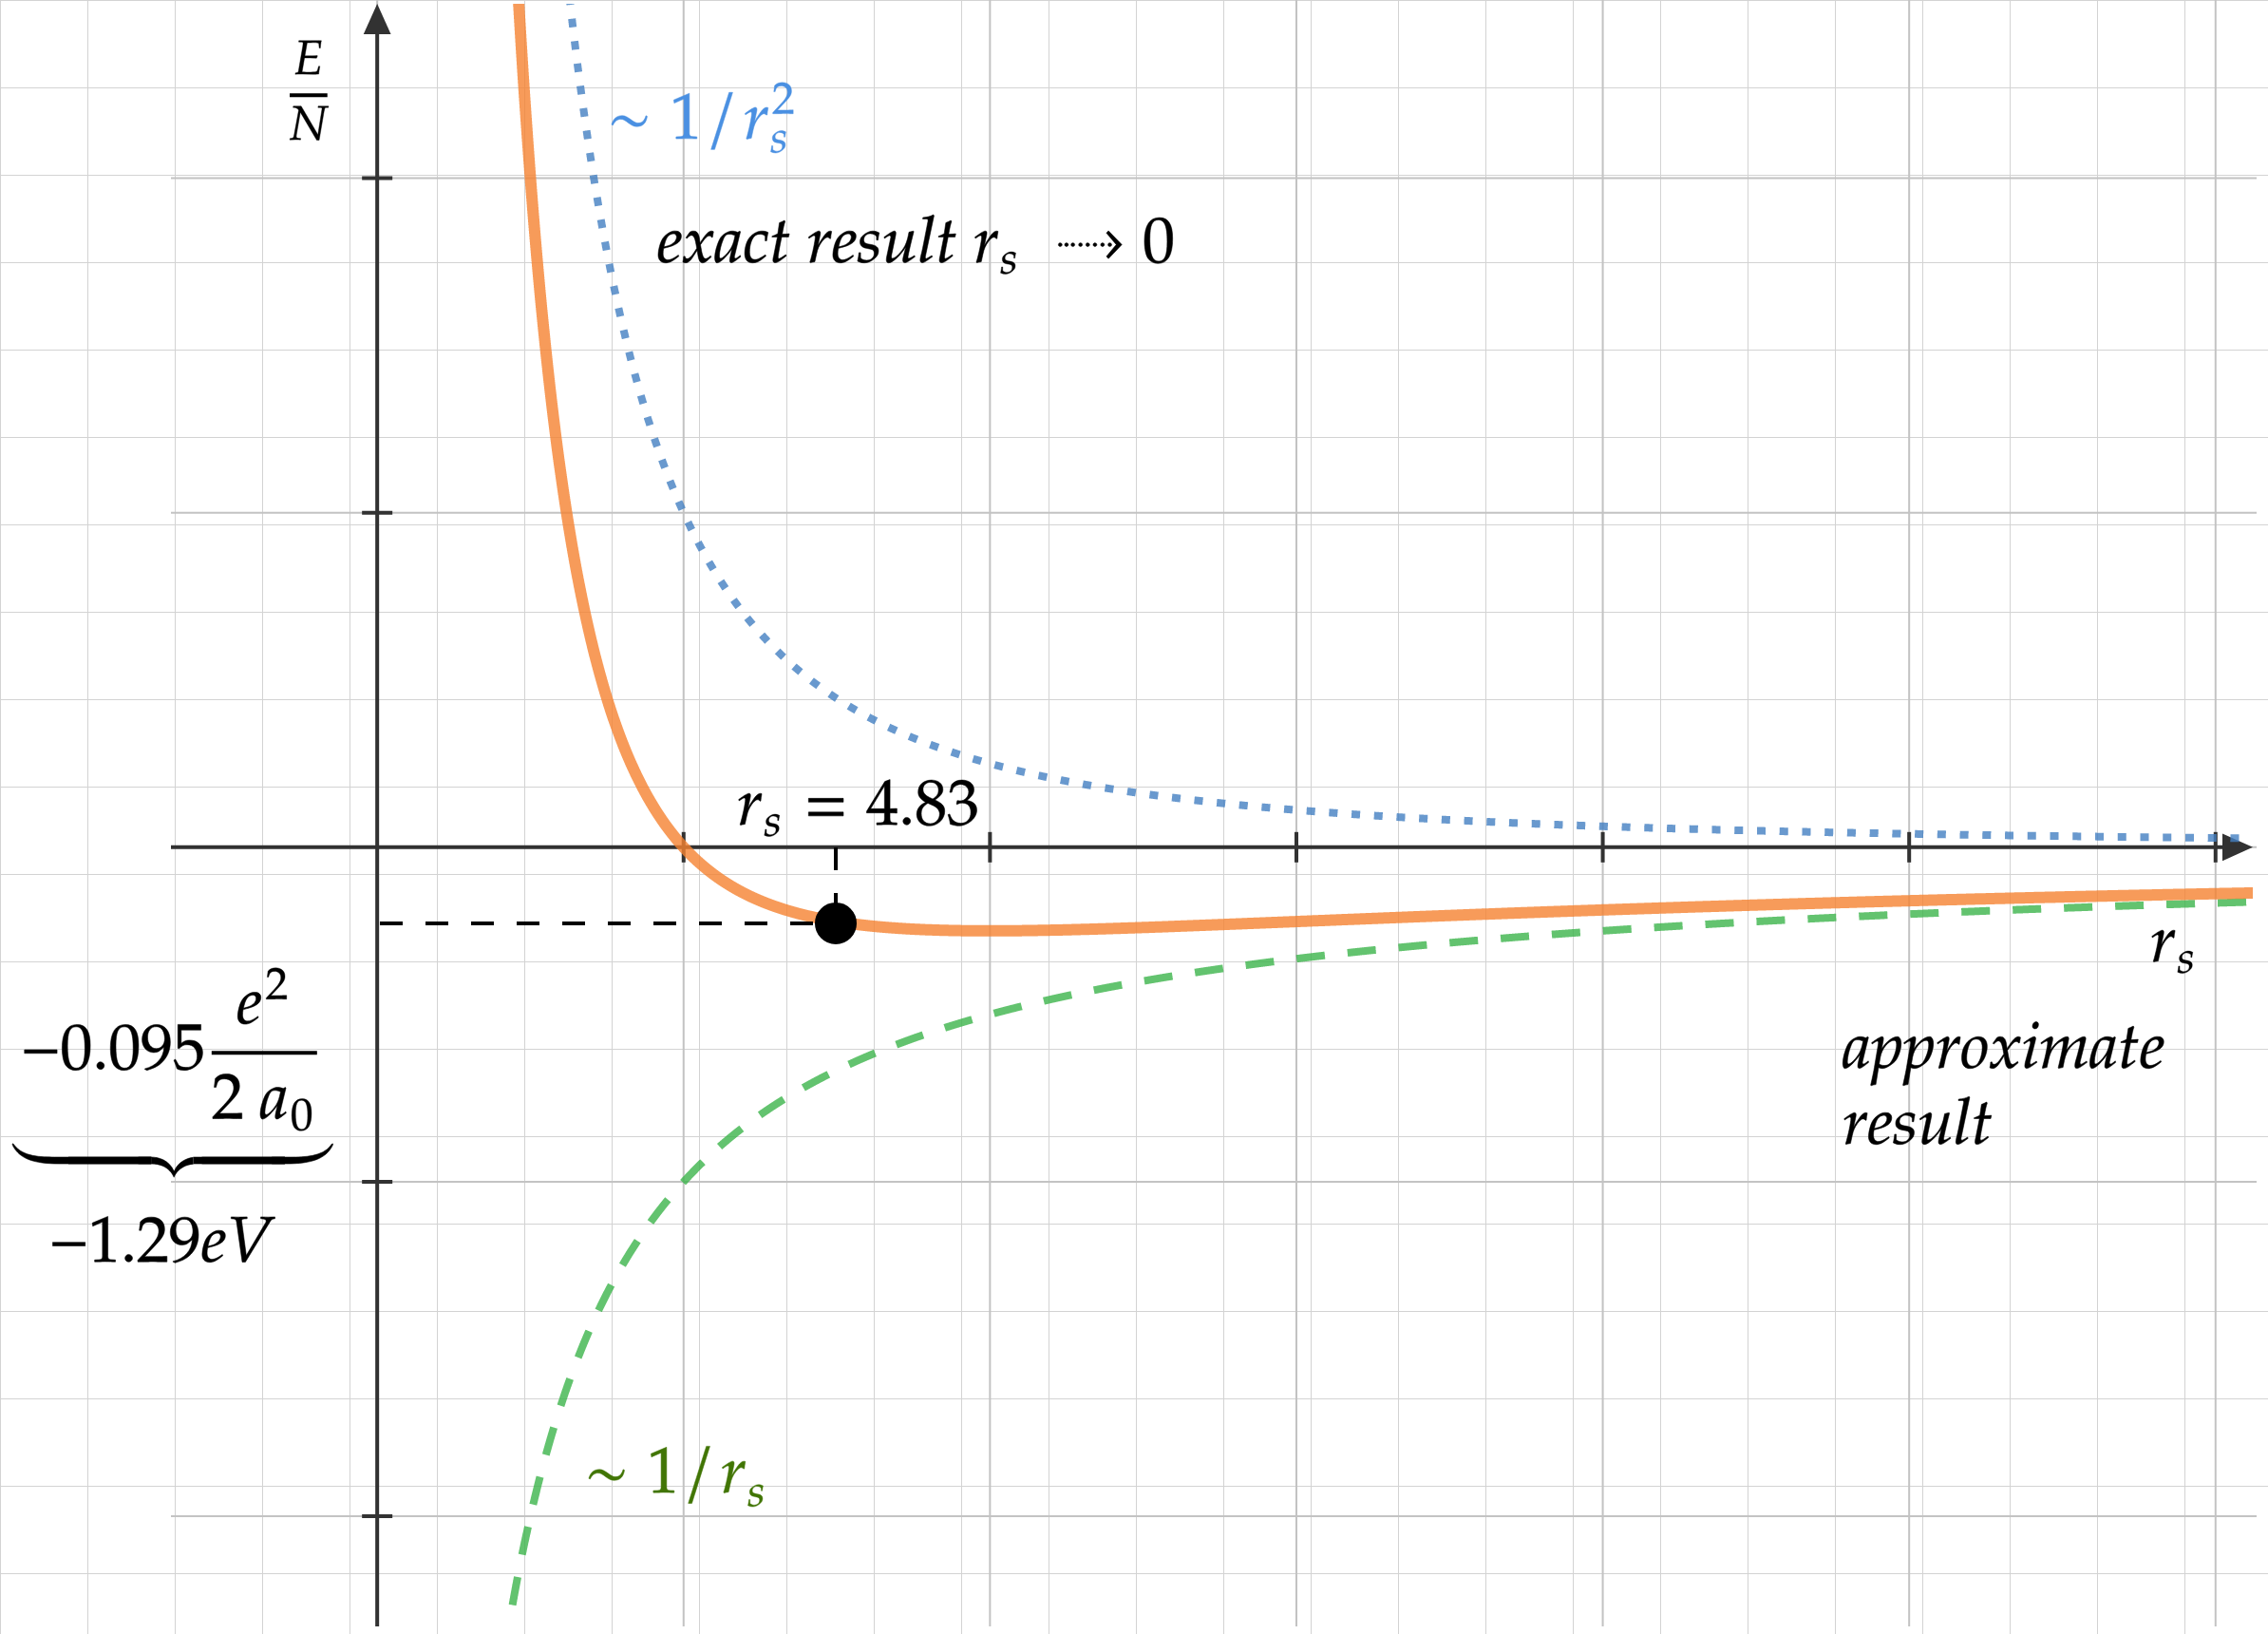
\includegraphics[width=0.7\textwidth]{../lessons/6_image/7.png}
\caption{\label{fig:6_4} Energy per particle at the first order.}
\end{figure}

For resuming, as \( r_s \rightarrow 0 \), high density limit, this is the exact solution, while for larger values of \( r_s \) the solution is only approximate. However, by using the \textbf{variational principle}:
\begin{equation*}
  \bra{F} \hat{H} \ket{F} = \bra{F} \hat{H}_0 + \hat{H}_1  \ket{F} \ge \bra{O} \hat{H} \ket{O}
\end{equation*}
it states that if we compute the Hamiltonian in the non-interacting ground state, by stopping at the first term of the perturbative expansion, the energy that we find is in any case higher or at most equal to the true ground state. Hence, our solution at the first order is an upperbound of the true solution!
Thus since already our solution gives a bound state, the true solution is even more bounded.

The exact solution certainly represents a bound system with energy lying below the approximated curve. As said, this explains why a metal is stable and this very simple model is able to explain the largest part of the binding energy of metals in a semi-quantitative way. For instance, let us consider Table \ref{table:6_1} in which we compare our results with the one obtained experimentally for the coesive energy of sodium. The correspondence is quite nice and the error is really small.
Therefore, the very important result is that we have a semi-quantitative agreement with experiments.

\begin{table}[h!]
\centering
\begin{tabular}{lll}
\toprule
  & \(r_s\) & \(E/N \,(eV)\) \\
\midrule
Na & 3.96 & -1.13 \\
Jellium model & 4.83 & -1.29 \\
\bottomrule
\end{tabular}
\caption{\label{table:6_1} Experimental results vs Jellium model.}
\end{table}

However, one should make some observation that in some sense reduce this good agreement:
\begin{itemize}
\item First of all, in our model there is nothing that has to do with the crystal lattice, so with the specific metallic system. One can show that for instance by comparing the results with experimental values for other metals the agreement is less good, so sodium is the best case that we can compare with.

\item Despite of the variational principle our extimated binding energy is lower than the experimental one \( E_{\text{Na}}> E_{jellium} \), due to the fact that we are neglecting a positive contribution to the kinetic energy due to the localized ions in real metals.

To make the situation clear, let us see the picture in Fig.\ref{fig:6_5} where the dashed line is the exchange contribution, the dotted line the kinetic contribution and the solid line the combination of the two. We can see that the binding energy of sodium is higher than our estimate, while from the variational principle we have expected the opposite. Of course we are neglecting some crucial features of real metals, that are characterized by not a smeared positive background, but by distribution of localized ions.
Since this ions are surrounded by core electrons, the valence electrons, that form the dynamical particles of the Jellium model, cannot go too close to these ions, so this means that they have roughly speaking less space to move in the system. Since this means that they should be a little more localized than in the Jellium model, more localization due to uncertainty principle means higher momentum.
In conclusion, in our model we are neglecting a positive contribution to the kinetic energy, which would make our solution higher in energy than our estimate.

\begin{figure}[h!]
\centering
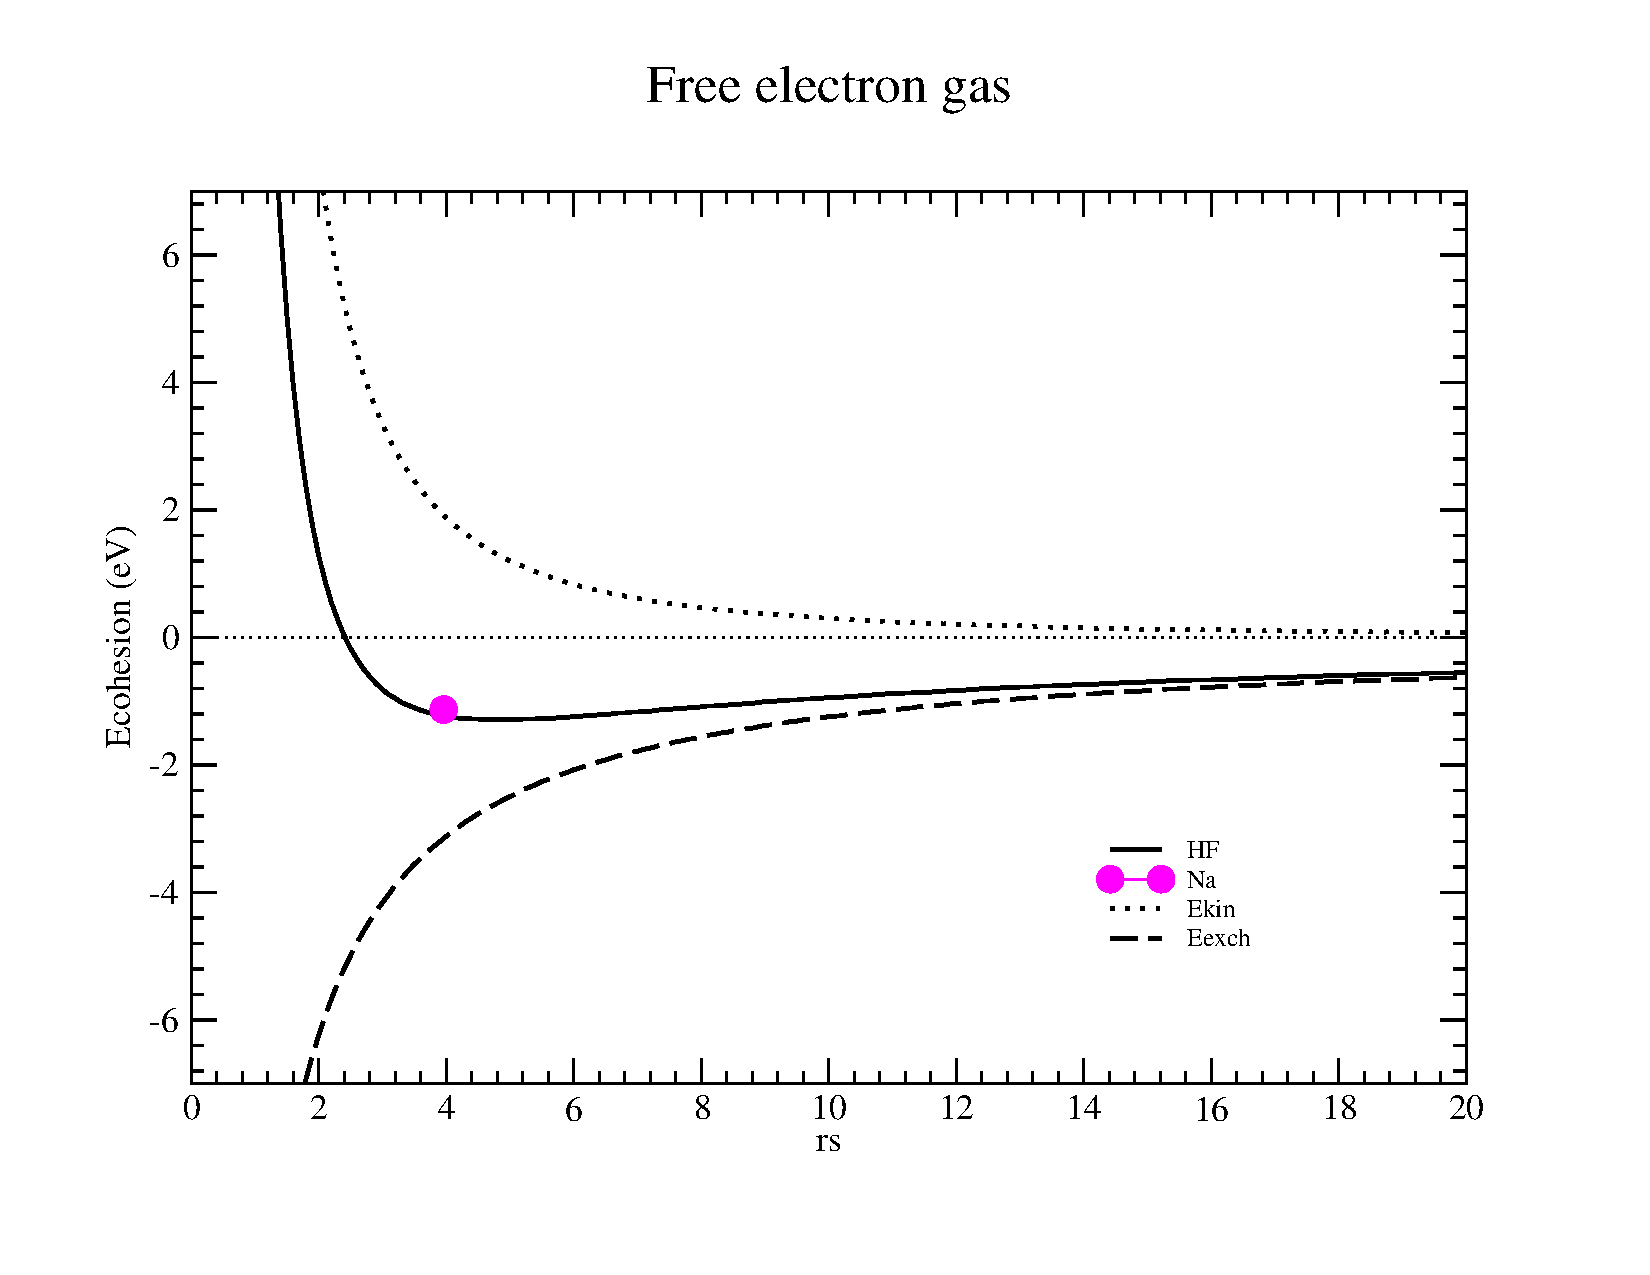
\includegraphics[width=0.7\textwidth]{../lessons/6_image/8.pdf}
\caption{\label{fig:6_5} Hartree-Fock energy.}
\end{figure}


\end{itemize}


Despite these observations, the one obtained is a very nice conclusion! Our very simple model is able to explain the most important contributions to the binding energy of real metals.

One could also think to go further improving the first order result by addition terms in the perturbative approach.
Unfortunately, if one tries to improve the \( 1^{st} \) order result by going to, for instance, \( 2^{nd} \) order perturbation theory, the result is disastrous: it diverges. It happens similarly for additionally terms. Hence, it is necessary some sort of \textbf{regularization} of the divergent behavior by taking higher order perturbation terms into account; the wrong idea is that  by taking into account many terms in the perturbative approach, we are able to regularize these divergences. Actually, it is not enough even take a large number of perturbative terms and one has to consider perturbation theory to \textbf{infinite order} (i.e. an infinite number of terms), which is not possible using standard perturbative approach, but we have to exploit all the possibilities of the quantum field theory. First of all, we will need to introduce some technical tools to be able to afford such a problem.

\subsubsection{Wigner solid}

Up to now we have estimated the basic properties, as equilibrium density and energy, of the Jellium model considering in particular the high density limit, where the kinetic energy is the dominant term.
One can also wonder what happens considering the opposite limit: the low density case \( r_s \rightarrow \infty  \). \marginpar{Low density limit} One can show (Wigner, 1938) that a lower energy (than that of the Jellium model) can be obtained by allowing the electrons to "crystallize" in a so called \textbf{Wigner solid}. Hence, instead of being free to move above the homogeneous background, electrons are  localized in a crystal of negative charges.

In fact, if the density is low there is a lot of space available for electrons and the zero-point kinetic energy associated with localizing the electrons becomes negligible in comparison with the electrostatic energy of a classical lattice of charges. Since essentially the electrons are very far from each other and are localized around lattice site, actually the quantum mechanical description is no longer essential because we can treat the particles as classical charged particles in a lattice.
Then, for instance the energy can be evaluated, despite of the long-range nature of the Coulomb interaction, by using methods used in solid state theory as for instance the Madelung-Ewald method in ionic solid.


\begin{remark}
Since from the variational principle we know that the true energy has a energy lower than the Jellium model energy and since in this case we get for large \( r_s \) a solution which is lower in energy than that obtained for the Jellium model, the Wigner solution is better than the Jellium one.
\end{remark}

The details of the derivation has been done by Wigner and we illustrate only the final conclusion. Thus, in the limit of low density, the energy per particle is given by:
\begin{equation*}
  \frac{E}{N} \underset{r_s \rightarrow \infty }{=} \qty(\frac{e^2}{2 a_0}) \qty[-\mathcolorbox{yellow!40}{\frac{1.79}{r_s}} + \mathcolorbox{green!20}{\frac{2.66}{r_s^{3/2}}} + \dots]
\end{equation*}
where the yellow term is obtained as the difference between the potential of the electrons on fixed lattice sites and the exchange energy\footnote{Remember that also for the Jellium model the exchange energy goes as the inverse of \( r_s \).}, while the green term is the zero-point oscillation of electrons about their equilibrium positions (i.e. electrons are forces to remain close to their lattice positions, but they can oscillate around these positions).

Summarizing, we have obtained two estimates of energy per particle in such a model, one for high density and one for low density. To be more precise:
\begin{itemize}
\item in the Jellium model the kinetic term dominates and it is valid for very high density: \( r_s <1 \).

\item in the Wigner-solid model the electrostatic potential energy term dominates and it is valid for very low density: \( r_s > 20 \).
\end{itemize}

Unfortunately, the region which is more interesting from a physical point of view is the one which corresponds to the densities of real metals and it is intermediate between these two cases: \( 2 < r_s < 6 \). In particular, in this region the kinetic and potential energy are comparable. This is clear from Fig.\ref{fig:6_5}, in which in the region from \( 2 \) to \( 6 \) both the kinetic energy and the exchange energy really are comparable.

In practice, it means that, as we will see better in the future, one needs to interpolate between high and low density to try to reproduce the behavior of real metals.

In conclusion, despite of the simplicity of the Jellium model, this is an interesting example in which we can apply the second quantization formalism and it is also interesting from a physical point of view for describing real metals.

Now, we skip to chapter 4 of the \cite{fetter} to try to develop the important formalism and tools that are required to go further in the perturbative approach. Hence, we do not deal with chapter 2, which is a summary of the basic notions of quantum statistical mechanics but we strongly suggest to read this chapter, because we will need some basic concepts of quantum statistical mechanics in the future.






\end{document}
